% v2-acmlarge-sample.tex, dated March 6 2012
% This is a sample file for ACM large trim journals
%
% Compilation using 'acmlarge.cls' - version 1.3, Aptara Inc.
% (c) 2011 Association for Computing Machinery (ACM)
%
% Questions/Suggestions/Feedback should be addressed to => "acmtexsupport@aptaracorp.com".
% Users can also go through the FAQs available on the journal's submission webpage.
%
% Steps to compile: latex, bibtex, latex latex
%
\documentclass[acmtap]{acmlarge}

% Metadata Information
\acmVolume{2}
\acmNumber{3}
\acmArticle{1}
\articleSeq{1}
\acmYear{2010}
\acmMonth{5}

% Package to generate and customize Algorithm as per ACM style
\usepackage[ruled]{algorithm2e}
\usepackage{graphicx}
\usepackage{listings}
\usepackage{amsmath}
\SetAlFnt{\algofont}
\SetAlCapFnt{\algofont}
\SetAlCapNameFnt{\algofont}
\SetAlCapHSkip{0pt}
\IncMargin{-\parindent}
\renewcommand{\algorithmcfname}{ALGORITHM}

% Page heads
\markboth{S. Sammak}{ME2055 Homework No. 6 \( \Delta t= 0.2.\) }

% Title portion
\title{ME2055 Homework No. 6}
\author{Shervin Sammak \affil{University of Pittsburgh}
}
% NOTE! Affiliations placed here should be for the institution where the
%       BULK of the research was done. If the author has gone to a new
%       institution, before publication, the (above) affiliation should NOT be changed.
%       The authors 'current' address may be given in the "Author's addresses:" block (below).
%       So for example, Mr. Fogarty, the bulk of the research was done at UIUC, and he is
%       currently affiliated with NASA.

\begin{abstract}
This homework provides a overview of numerical solutions to the nonlinear hyperbolic equation known as Burger equation. The Lax, Lax-Wendroff, MacCormack and Beam and Warming implicit schemes are developed, and applied to a inviscid burger equation.  The results of running the
codes on different CFL numbers is demonstrated. These simple calculations show that the how explicit and implicit schemes converged to results and how dissipation and dispersion error propagates in the domain. 
\end{abstract}

\category{}{ME2055- Spring 2014}{}

% At a minimum you need to supply the author names, year and a title.
% IMPORTANT:
% Full first names whenever they are known, surname last, followed by a period.
% In the case of two authors, 'and' is placed between them.
% In the case of three or more authors, the serial comma is used, that is, all author names
% except the last one but including the penultimate author's name are followed by a comma,
% and then 'and' is placed before the final author's name.
% If only first and middle initials are known, then each initial
% is followed by a period and they are separated by a space.
% The remaining information (journal title, volume, article number, date, etc.) is 'auto-generated'.

\begin{document}



\maketitle

% Head 1
\section{Introduction}

The inviscid burger equation is
\begin{eqnarray}
\frac{\partial U(x,t)}{\partial t} + U(x,t) \frac{\partial U(x,t)}{\partial x} &=& 0
\end{eqnarray}
which, may be expressed as 

\begin{eqnarray}
\frac{\partial U(x,t)}{\partial t} + \frac{1}{2} \frac{\partial {{U(x,t)}^{2}} }{\partial x} &=& 0
\end{eqnarray}
Two different cases are investigated. To differ between these to cases, \(U\) and \(U^\prime\) are used respectively.
In first case:
\(t \in [0, 2.4]\) is time; \(x \in [0, 40]\) is the spatial variable; \(U = U(x,t)\) is the velocity. To make the differential equation well settled, I need to give initial condition.

\begin{eqnarray}
U(x,0) &=& 5.0;  \qquad \mbox{for } x \in [0,20]  \nonumber \\
U(x,0) &=& 0.0;  \qquad  \mbox{for } x \in (20,40]. 
\end{eqnarray}

In the second case initial velocity distribution is given by the following:

%\begin{eqnarray}
\[ U ^\prime (x,0) = \left\{
  \begin{array}{l l}
    1 & \quad x \in [0,0.25]\\
    1.25 - x & \quad x \in (0.25,1.25]\\
    0 & \quad x \in (1.25,4]
  \end{array} \right.\]
%\end{eqnarray}
The spatial domain is  \(x \in [0, 4]\) and the solution is sought up to 6.0 seconds. boundary conditions are simply specified as 
\begin{eqnarray}
U^ \prime (0.0, t) = 1.0 \nonumber \\
U^ \prime (4.0, t)= 0.0.
\end{eqnarray}
% Head 2
\section{Schemes for the Burger Equation}
The gird for the discretization is:
\begin{eqnarray}
\Delta t &=&  0.1, \ 0.2 \nonumber \\
\Delta x &=&  1.0. \\
\Delta t ^ \prime &=&   0.01, \ 0.025, \ 0.05, \ 0.1  \nonumber \\
\Delta x ^ \prime &=&  1.0 .
\end{eqnarray}

For convenience, I denote \(U(x_{m}, t_{n})\) and \(U ^ \prime (x_{m}, t_{n})\) as \(U_{m}^{n}\) and \({U ^ \prime}_m^n   \). Then I state the numerical method. \\
\subsection{Lax Method}
This explicit method uses forward time differencing and central space differencing with the order of \([(\Delta t), ({\Delta x}^2)]\). The corresponding FDE for Eq. (1) is
\begin{eqnarray}
U_{m}^{n+1} &=& U_{m}^{n} +\frac{1}{2} (U_{m+1}^{n}+ U_{m-1}^{n}) - \frac{\Delta t}{4 \Delta x} ({U_{m+1}^{n}}^2- {U_{m-1}^{n}}^2)
\end{eqnarray}

\subsection{Lax-Wendroff Method}
The Lax-Wendroff method is second order scheme with a stability requirement of \(|U_{max} \frac{\Delta t}{\Delta x} | < 1\). The finite difference equation for this scheme is

\begin{eqnarray}
U_{m}^{n+1} &=& U_{m}^{n} - \frac{\Delta t}{2 \Delta x} (E_{m+1}^{n}- E_{m-1}^{n}) \nonumber \\ &+& \frac{{\Delta t}^2}{4 {\Delta x}^2} [(U_{m+1}^{n}+ U_{m}^{n})({E_{m+1}^{n}}- {E_{m-1}^{n}}) - (U_{m+1}^{n}+ U_{m}^{n})({E_{m+1}^{n}}- {E_{m-1}^{n}})].
\end{eqnarray}

wherein; \(E=\cfrac{U^2}{2}\).
\subsection{MacCormack Method}
This multi-level method applied to the Eq. (1) yields two FDEs.

\begin{eqnarray}
U_{m}^{*} &=& U_{m}^{n} - \frac{\Delta t}{ \Delta x} (E_{m+1}^{n}- E_{m}^{n}). \\
U_{m}^{n+1} &=& \frac{1}{2}(U_{m}^{n} + U_{m}^{*}) - \frac{\Delta t}{2 \Delta x} (E_{m}^{*}- E_{m-1}^{*}).
\end{eqnarray}



The stability condition is the same as for Lax-Wendroff method.


\subsection{Beam and Warming Implicit Method}
Implicit formulation of Beam and Warming has second-order accuracy which is unconditionally stable.
This approximation applied to model equation (Eq. (1)) yields:

\begin{eqnarray}
-\frac{\Delta t}{4 \Delta x}U_{m-1}^{n} U_{m-1}^{n+1} + U_{m}^{n+1} + \frac{\Delta t}{4 \Delta x}U_{m+1}^{n} U_{m+1}^{n+1} &=& U_{m}^{n}  - \frac{\Delta t}{2 \Delta x}(U_{m+1}^{n}  - U_{m-1}^{n}) \nonumber \\ &+& \frac{\Delta t}{4 \Delta x}({U_{m+1}^{n}}^2 - {U_{m-1}^{n}}^2 ).
\end{eqnarray}

Once this equation is applied to all grid points at the unknown time level, a set of algebraic equations will result. These equations can be represented in a matrix form, where the coefficient matrix is tridiagonal.
The implicit method is just
\begin{eqnarray}
B\textbf{U}^{n+1} = \textbf{U}^{n} .
\end{eqnarray}

This is a process of solving linear system of equations at each time step. \\

\section{Results }
\subsection{Case I}
The solution for \( \Delta t= 0.1,0.2\) and  \( \Delta x=1\) at several time intervals is presented in Fig. (1), which clearly reflects that the dissipative nature of solution. Note that the discontinuity is illustrated over several grid points. As the \(\Delta t\) gets higher, the correspondent CFL number gets bigger and so the difference between numerical and exact solutions decreases. \\

\begin{figure}[htb]
  \centering
  \begin{tabular}{cc}

    % Requires \usepackage{graphicx}

    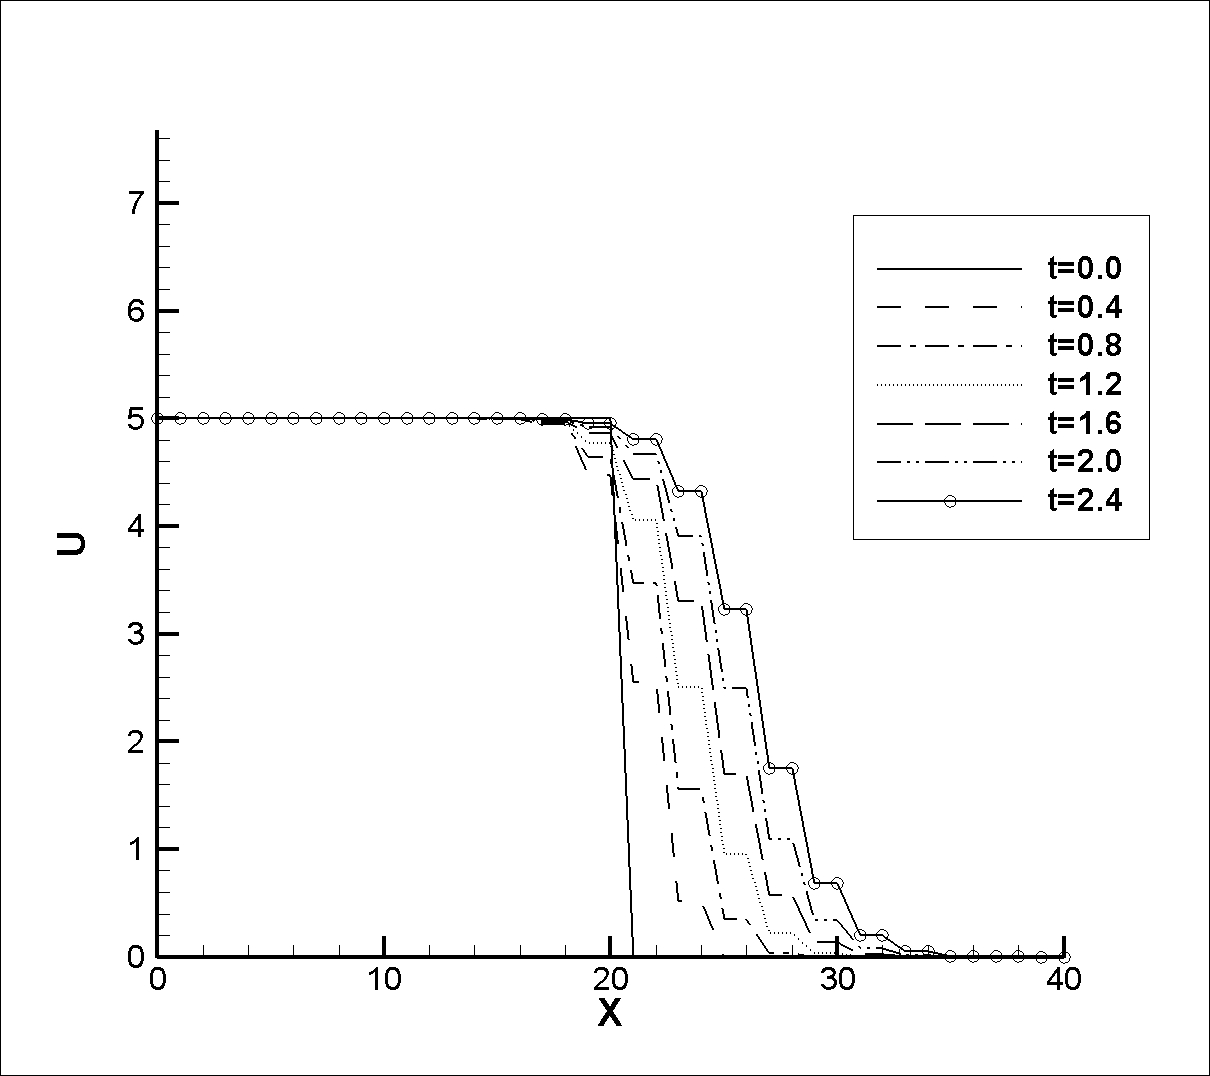
\includegraphics[width=80mm]{lax.jpg} 
    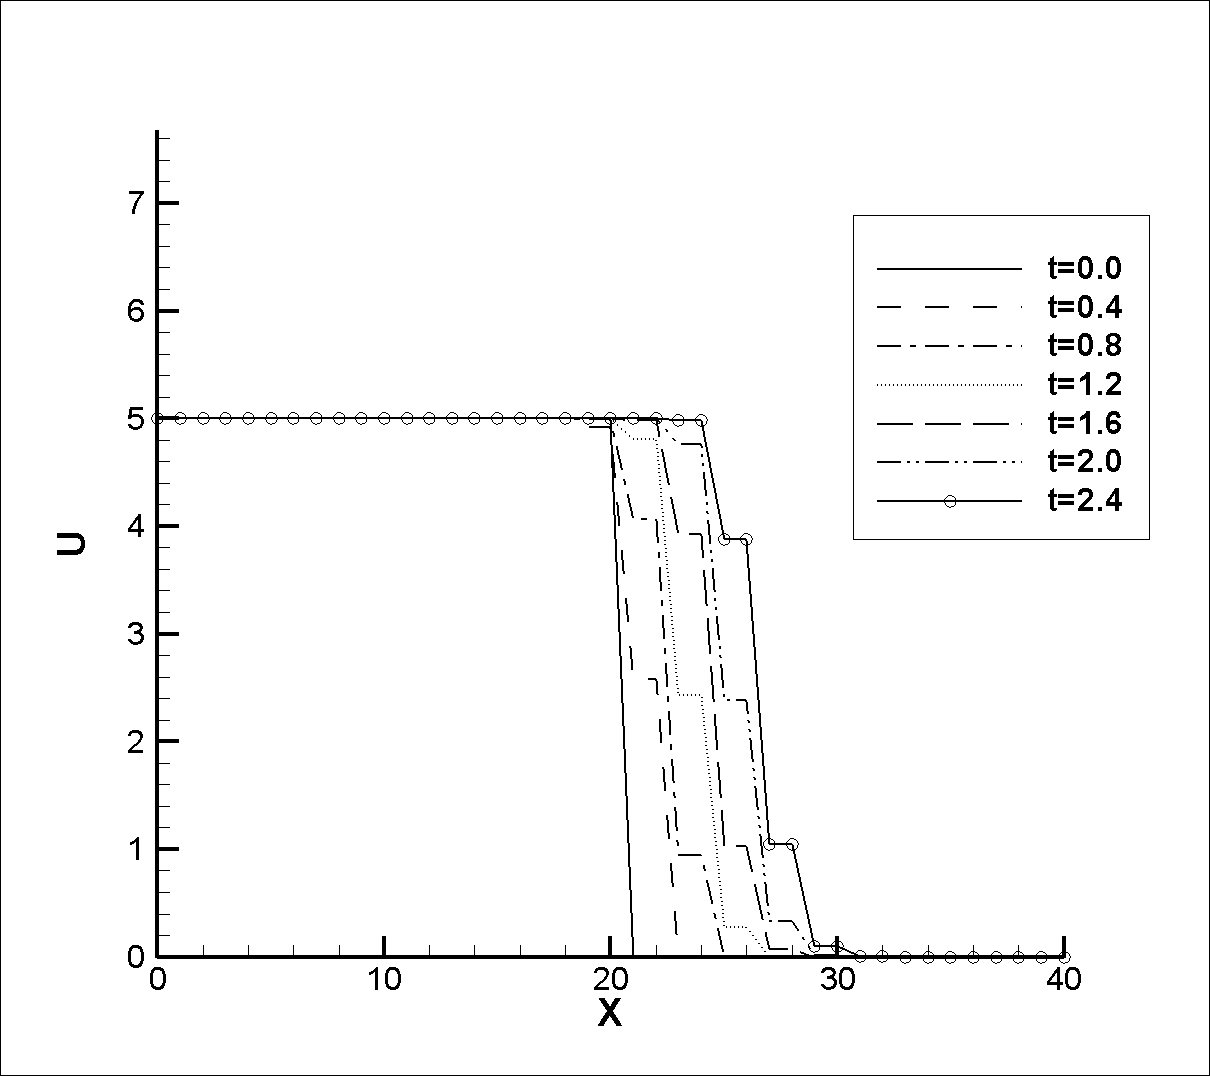
\includegraphics[width=80mm]{lax2.jpg} 


  \end{tabular}
\label{figur}\caption{(Solution of inviscid Burgers equation by the Lax method, left:\(\Delta t=0.1 \) and Right: \( \Delta t= 0.2.\)}
\end{figure}

For the Lax-Wendroff method, solution has a oscillation in the neighborhood of the discontinuity. As the CFL increases from 0.1 to 0.2 the magnitude of dispersion error gets smaller.

\begin{figure}[htb]
  \centering
  \begin{tabular}{c}

    % Requires \usepackage{graphicx}

    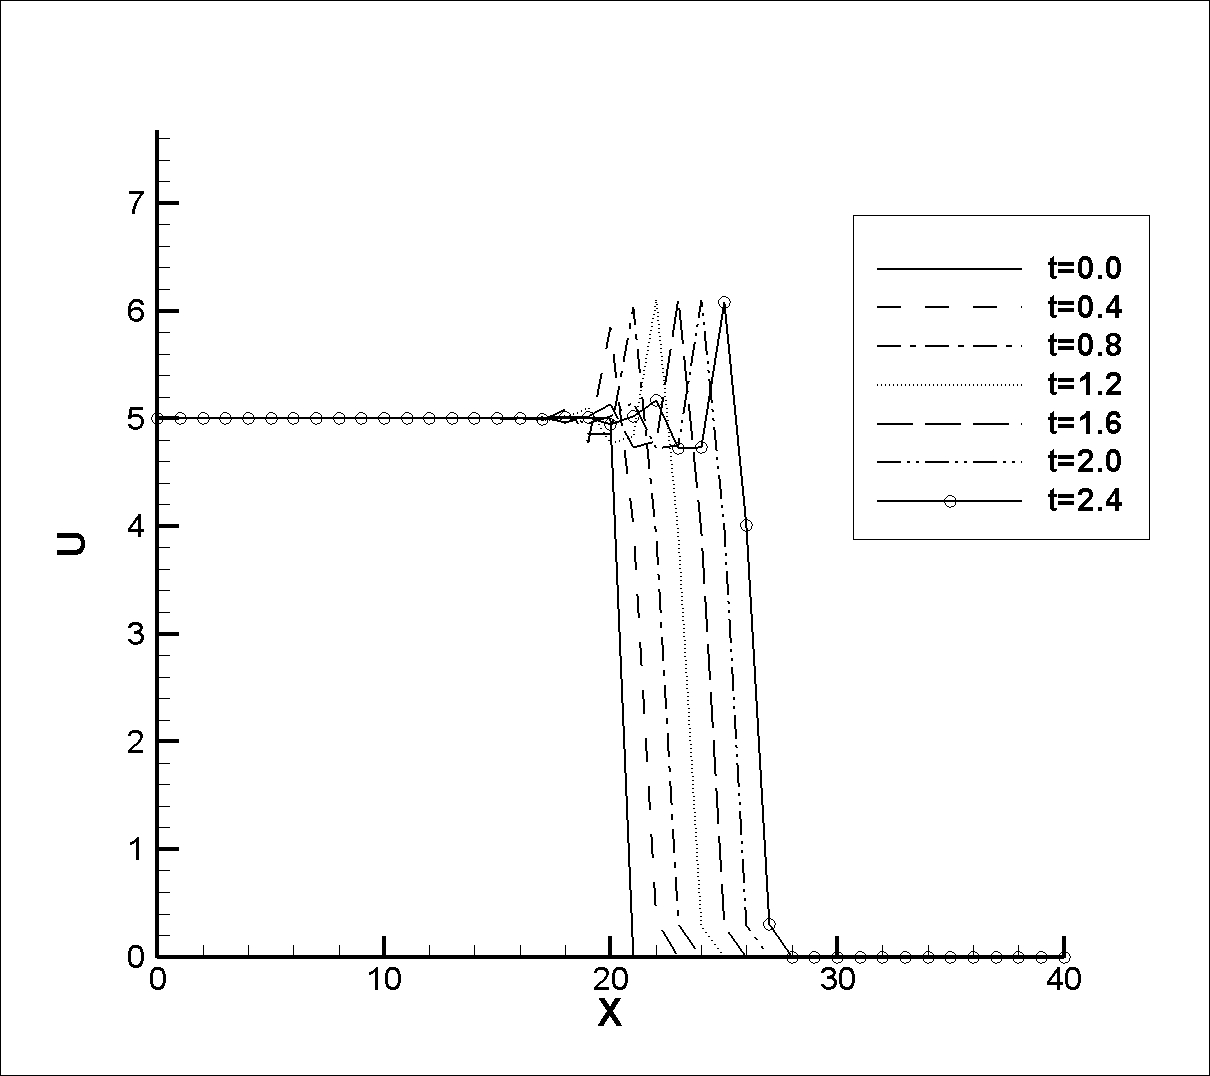
\includegraphics[width=80mm]{lw.jpg} 
    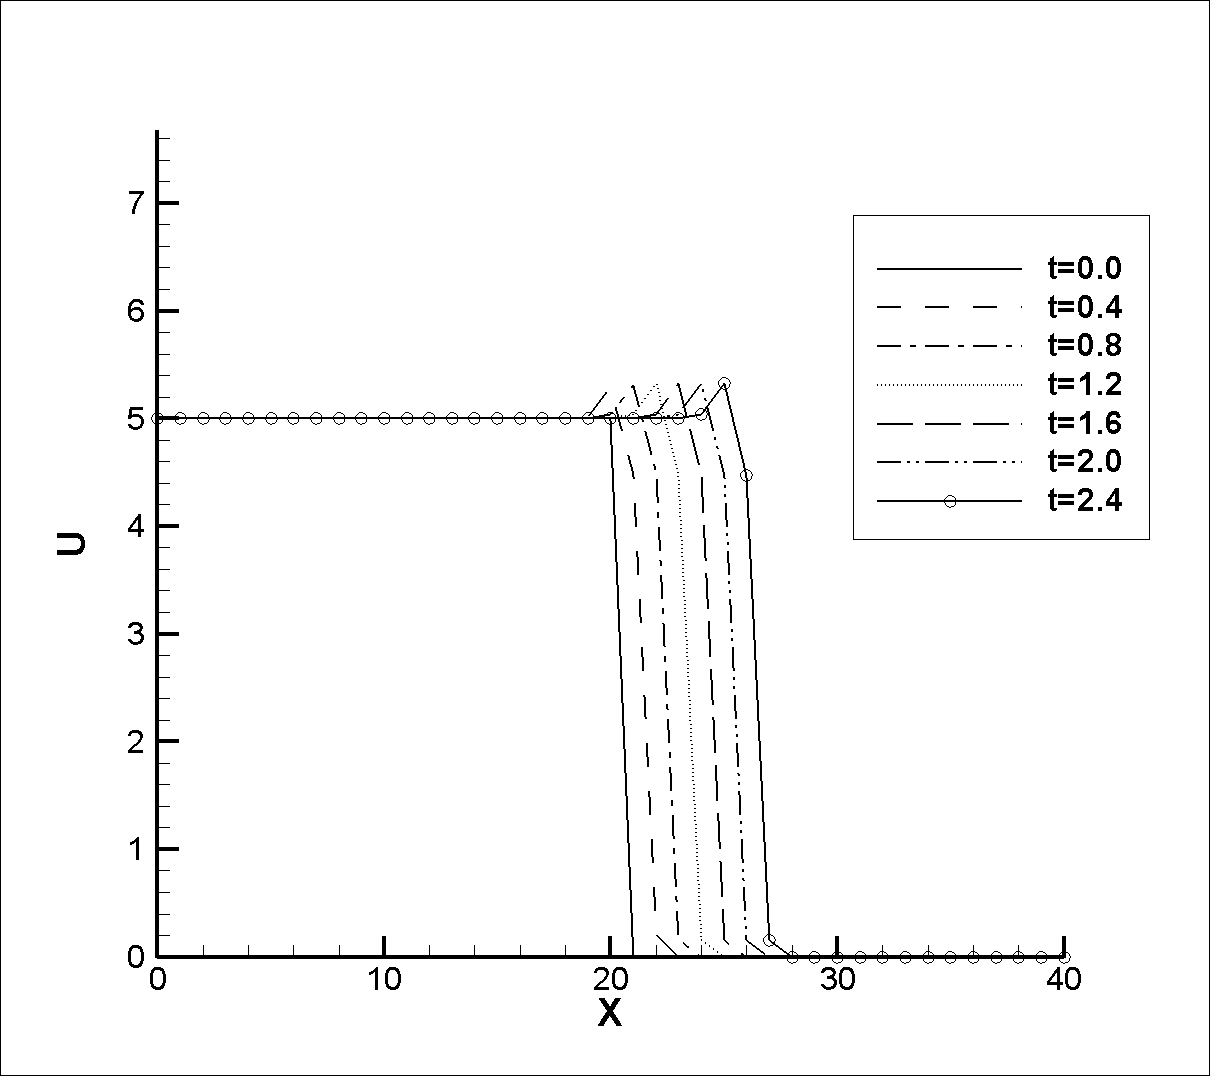
\includegraphics[width=80mm]{lw2.jpg} 


  \end{tabular}
\label{figur}\caption{Solution of inviscid Burgers equation by the Lax-Wendroff method, left:\(\Delta t=0.1 \) and Right: \( \Delta t= 0.2.\)}
\end{figure}

Unlike the Lax and Lax-Wendroff method, MacCormack scheme has better solution. Due to the prediction and correction step, the answer is well behaved. Furthermore, like the other method explicit methods, as the CFL number increases, the magnitude of error will reduce.

\begin{figure}[htb]
  \centering
  \begin{tabular}{c}

    % Requires \usepackage{graphicx}

    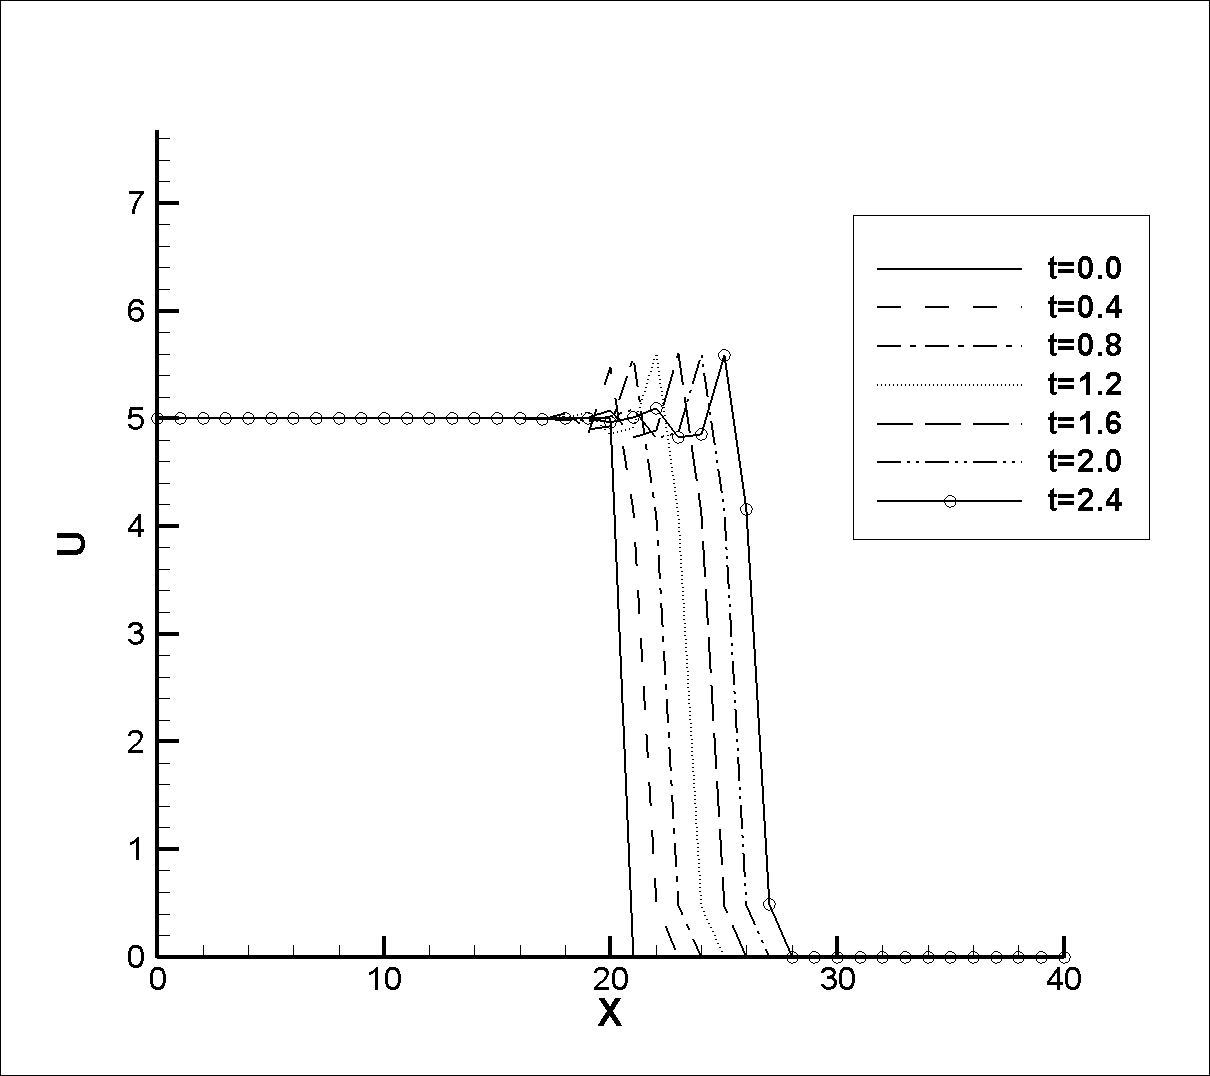
\includegraphics[width=80mm]{mac.jpg}
    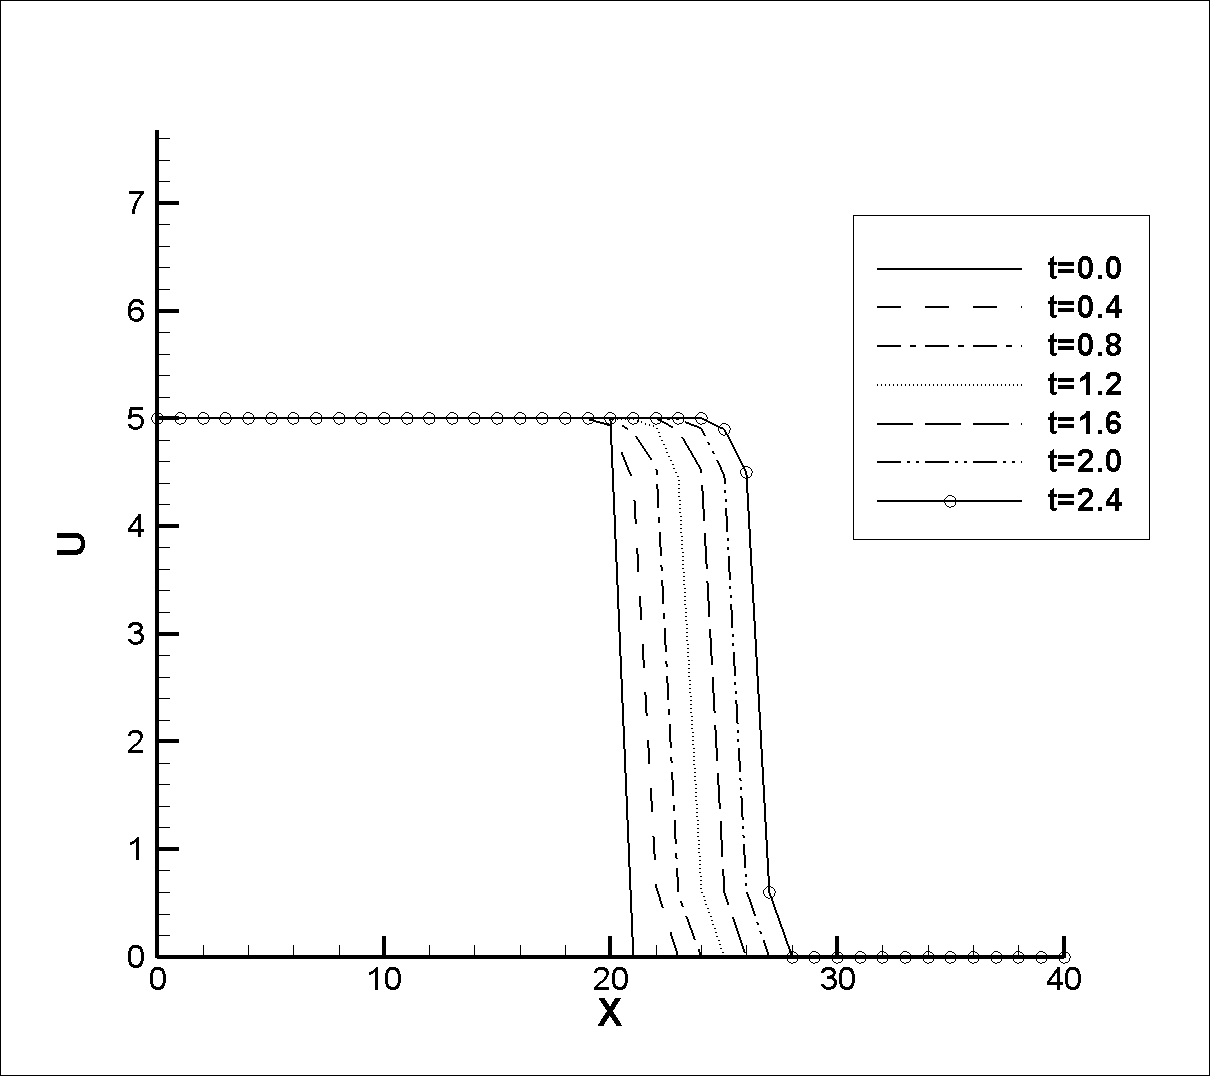
\includegraphics[width=80mm]{mac2.jpg}  


  \end{tabular}
\label{figur}\caption{Solution of inviscid Burgers equation by the MacCormack method, left:\(\Delta t=0.1 \) and Right: \( \Delta t= 0.2.\)}
\end{figure}
  
The solution of the implicit method at several time intervals is shown in Fig. (4). Beam and Warming scheme has a second-order accuracy and because of that, the dispersion error propagates and its amplitude gets higher over the time. 
Since for the larger time step size (higher CFL number) the dispersion error increases, some damping terms could be used to reduce the level of dispersion error. 

\begin{figure}[htb]
  \centering
  \begin{tabular}{c}

    % Requires \usepackage{graphicx}

    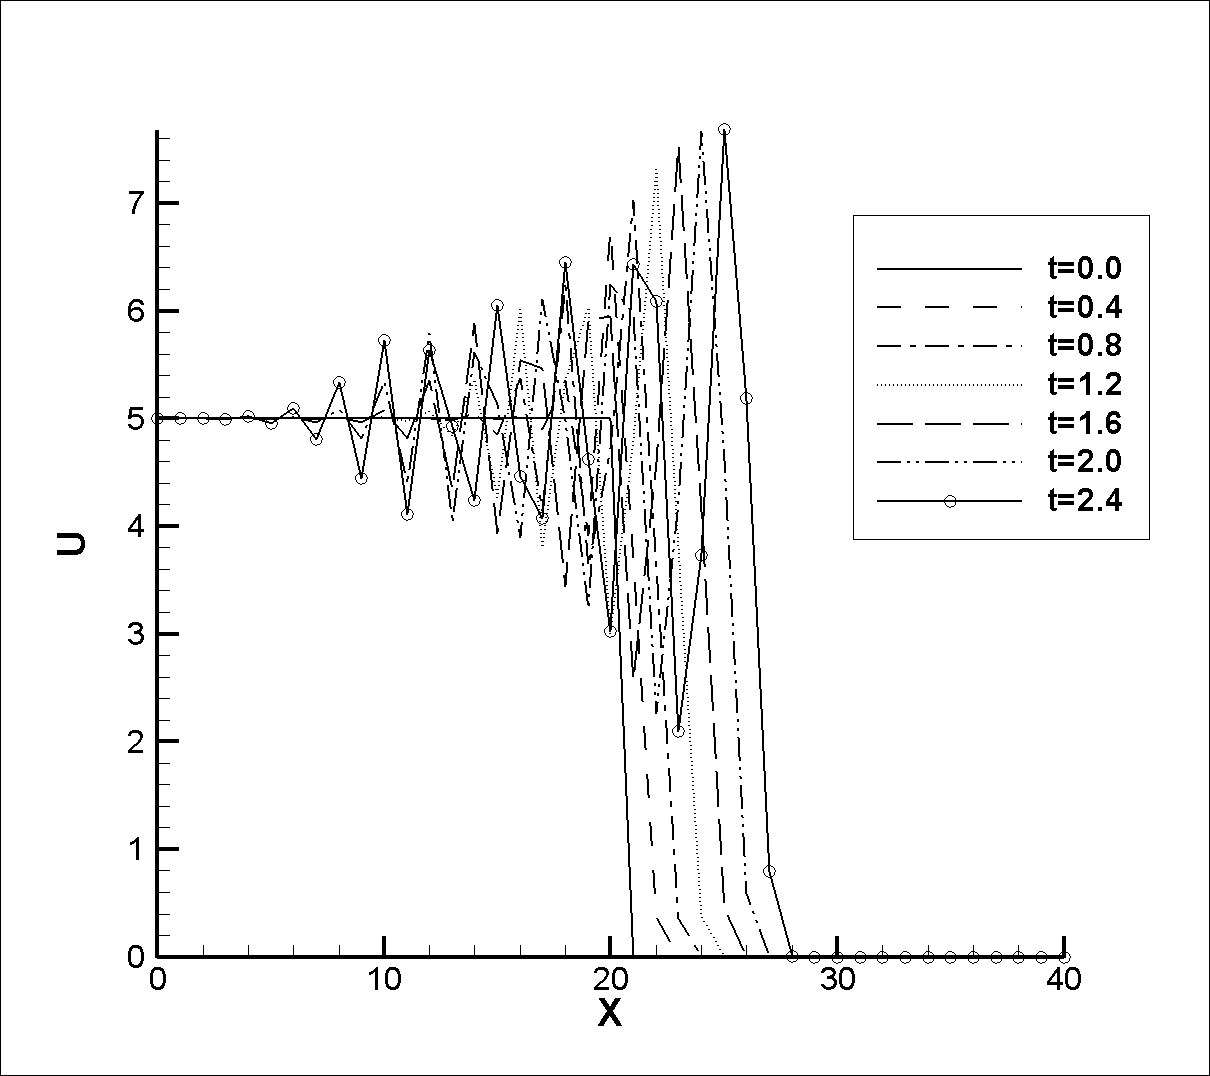
\includegraphics[width=80mm]{beam.jpg} 
    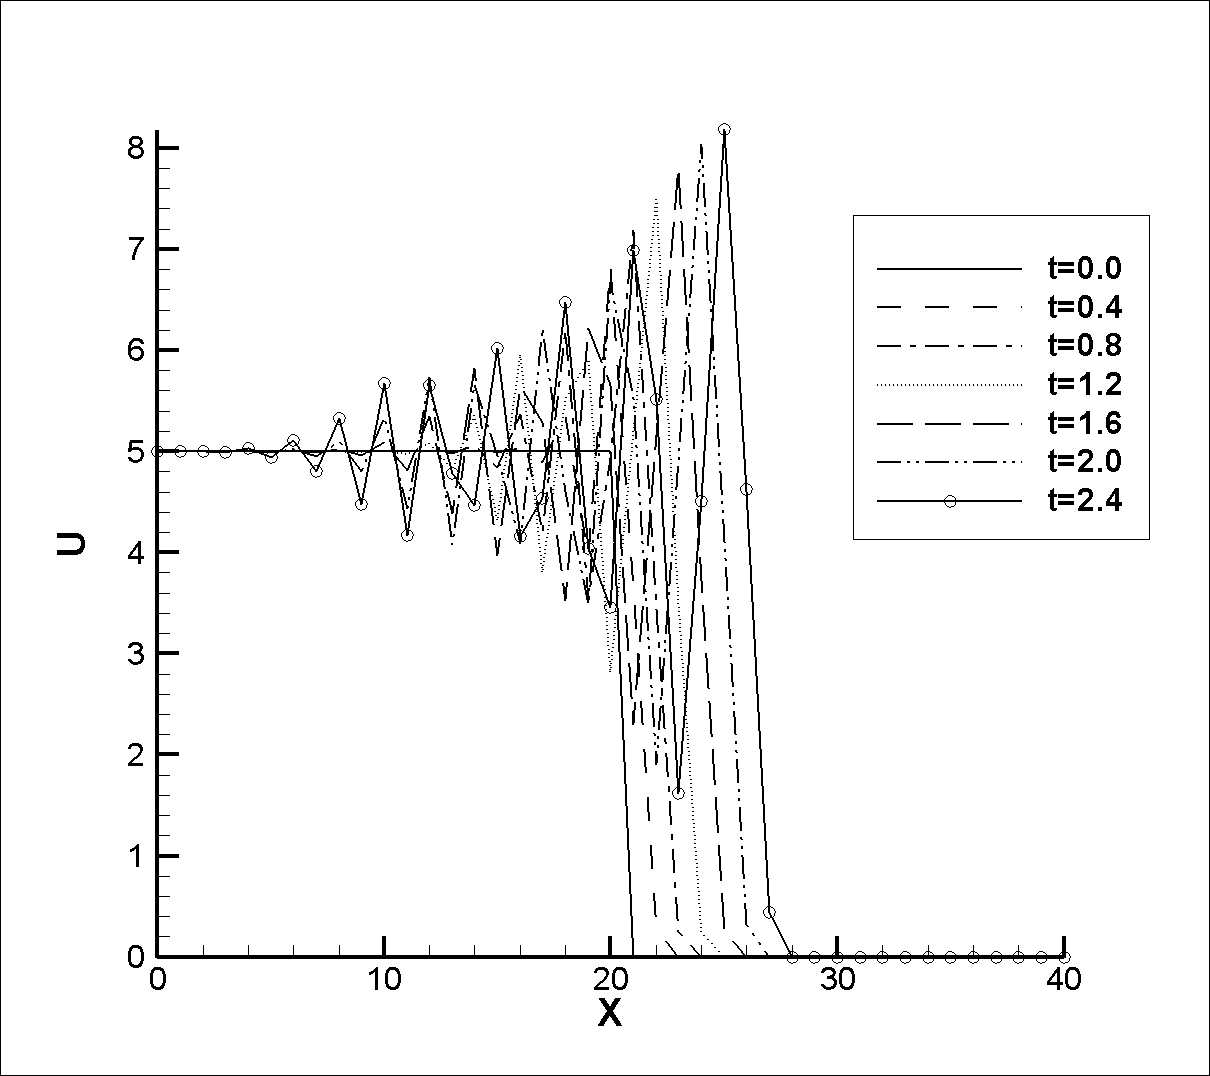
\includegraphics[width=80mm]{beam2.jpg} 


  \end{tabular}
\label{figur}\caption{Solution of inviscid Burgers equation by the Beam and Warming method, left:\(\Delta t=0.1 \) and Right: \( \Delta t= 0.2.\)}
\end{figure}


The solution behaves differently when Lax-Wendroff method is used. Since the algorithm is second-order accurate, some dispersion error is expected. Indeed, the oscillatory behavior of the solution for the smaller CFL number clearly indicates the error developed in the solution. Note that the amplitude of the solution remains the same.


\subsection{Case II}
In all three cases, dispersion error illustrated. In Fig. (5), the middle plot corresponds to CFL number equal to 1. In general, as the CFL number as the CFL number decreases, the solution degenerates; the best solution is obtained at CFL equal to unity. 


\begin{figure}[htb]
  \centering
  \begin{tabular}{c}

    % Requires \usepackage{graphicx}

    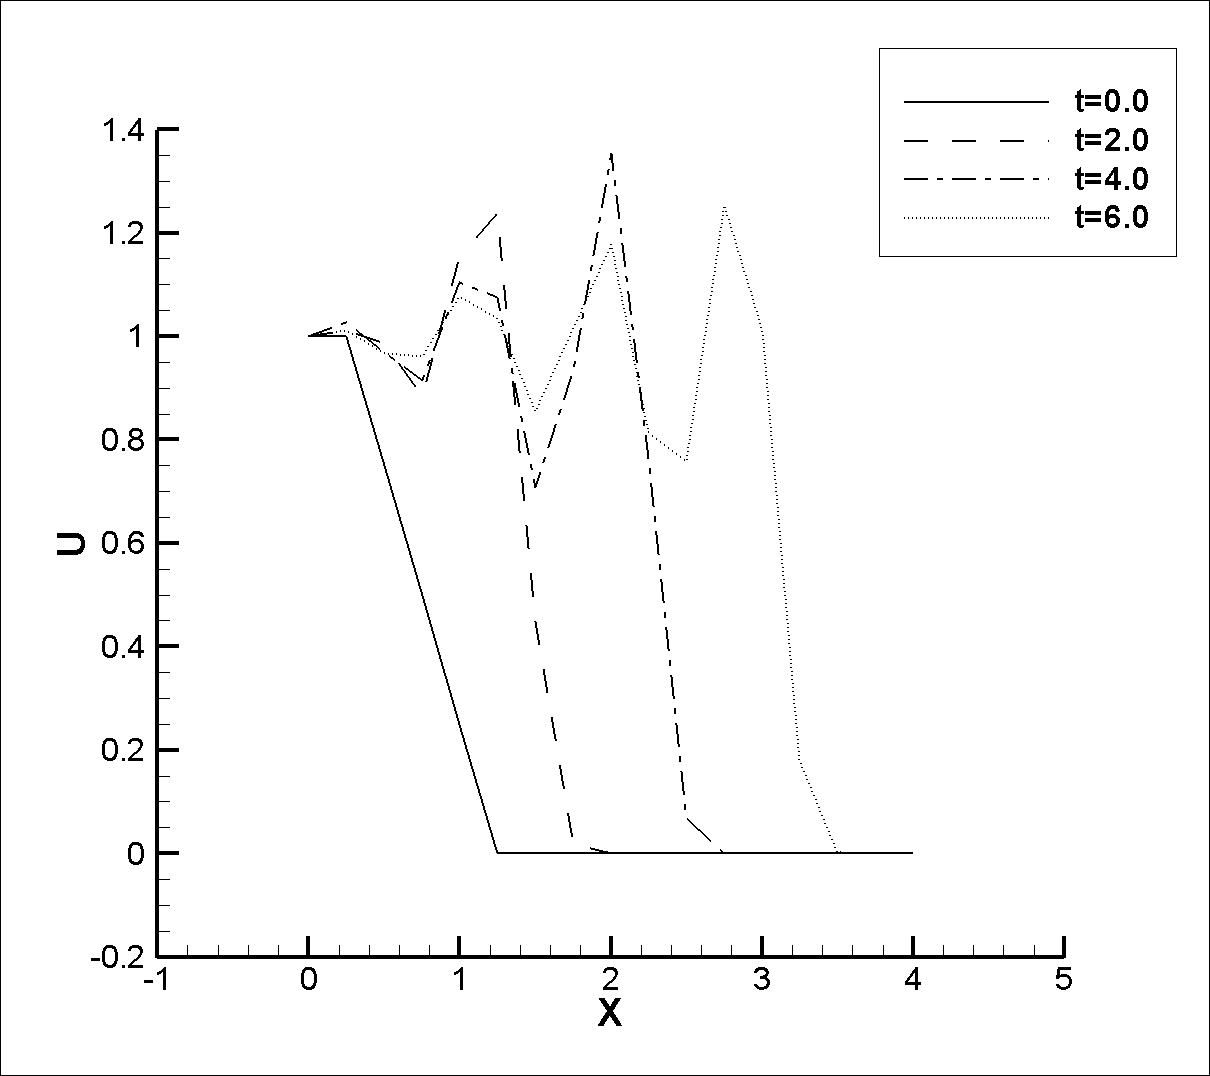
\includegraphics[width=50mm]{c2.jpg} 
    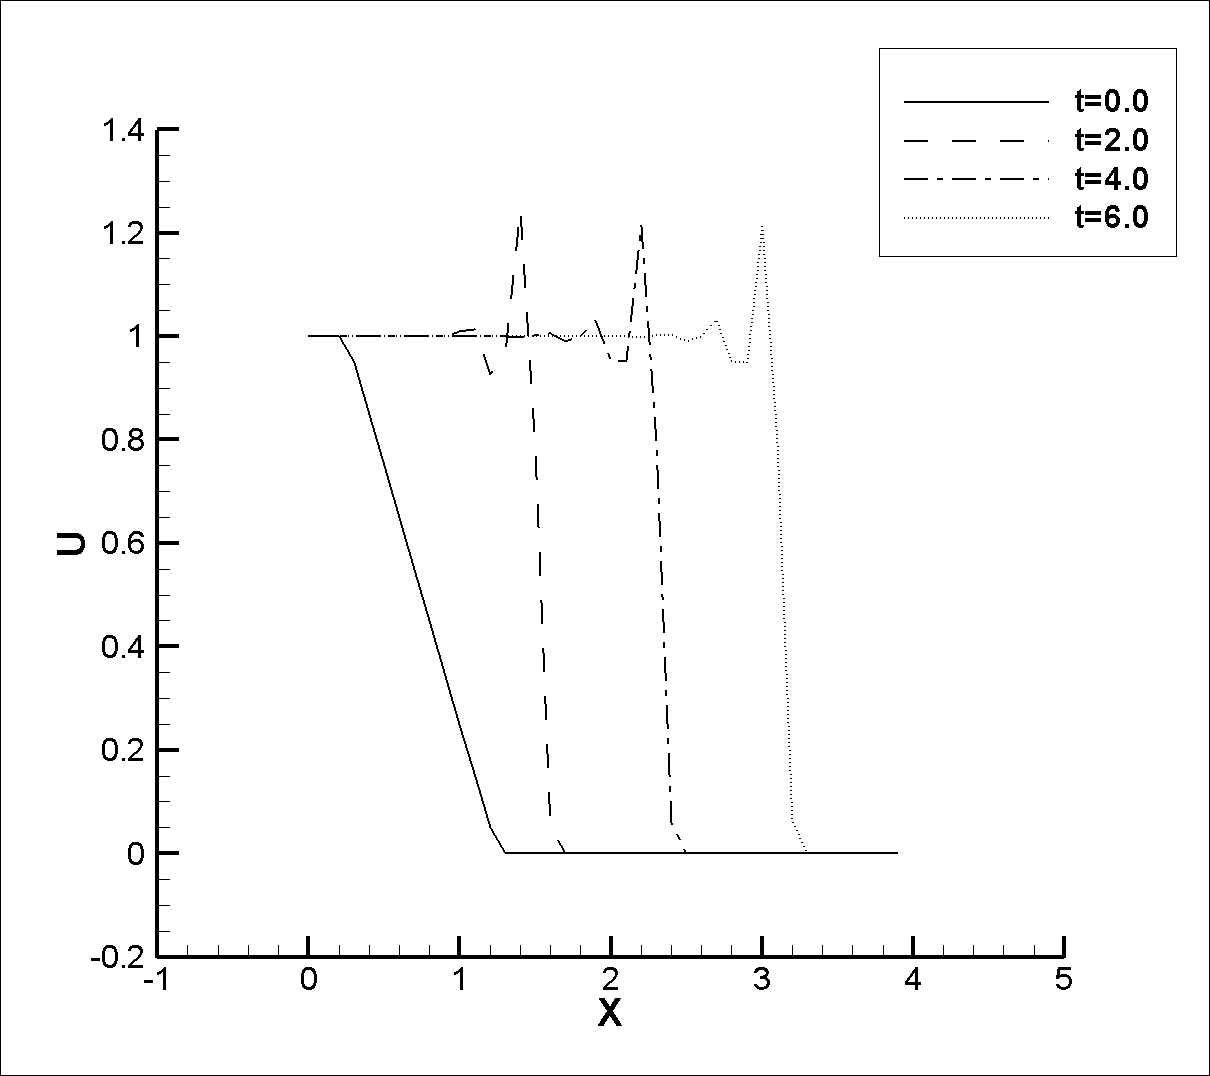
\includegraphics[width=50mm]{c05.jpg}
    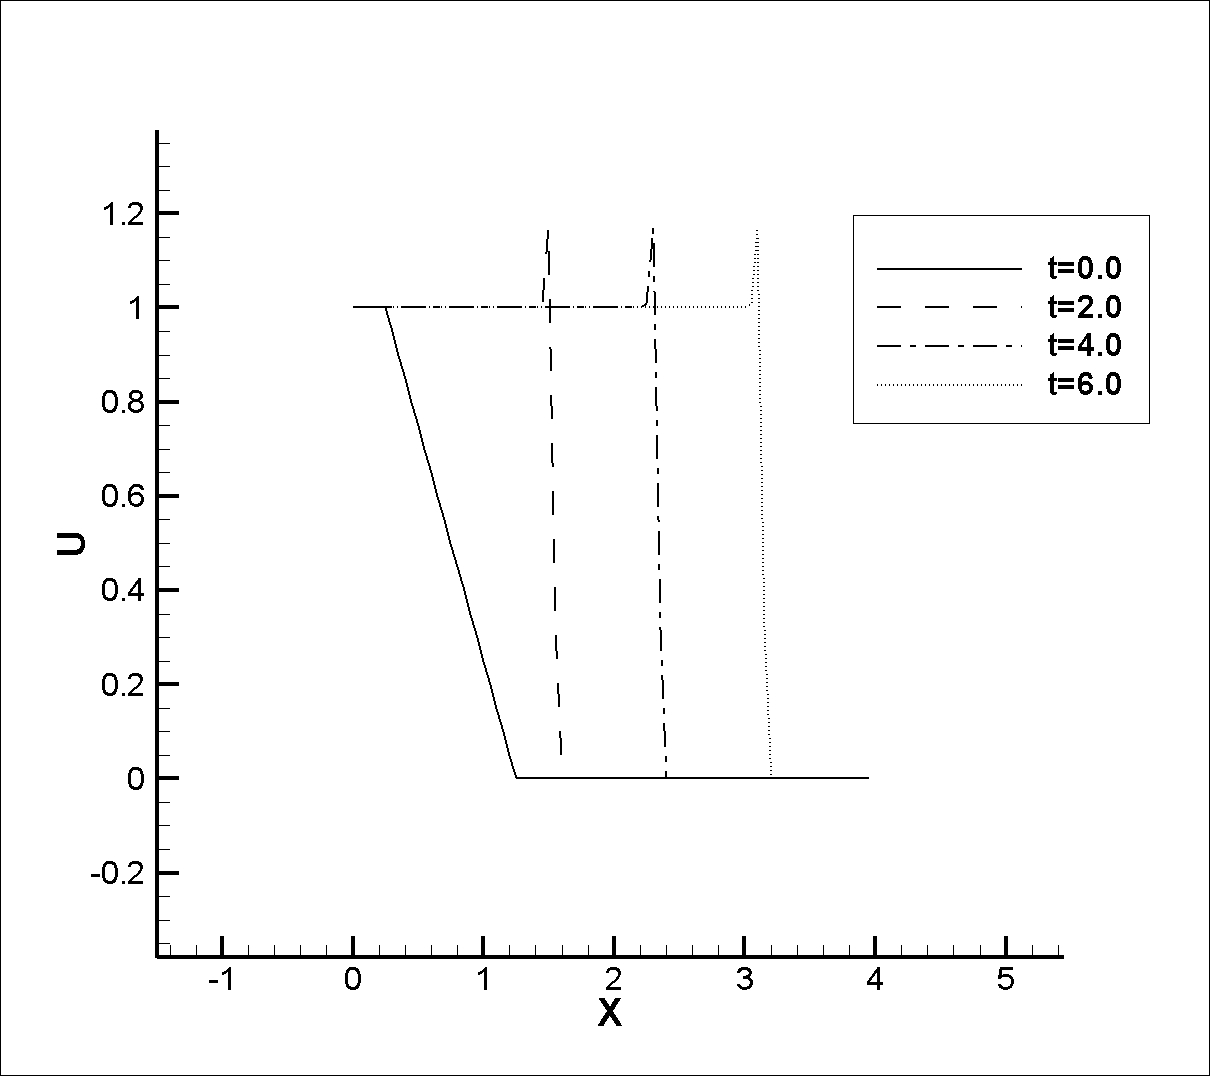
\includegraphics[width=50mm]{c1.jpg} 
    

  \end{tabular}
\label{figur}\caption{Solution of inviscid Burgers equation by Lax-Wendroff method, left:    \(\Delta t=0.025 \), middle: \(\Delta t=0.05 \)  and Right: \( \Delta t= 0.1.\)}
\end{figure}

For the stabilty condition in Lax-Wendroff method, \(|U_{max} \frac{\Delta t}{\Delta x} | < 1\) should be satisfied but for \(\Delta t= 0.1\), \(|U_{max} \frac{\Delta t}{\Delta x} | =2 \), so the solution will not converge for this case.

\section{Conclusion}
Again, the error is the smallest at the upper limit value of the CFL number, i.e., when the CFL number approaches one. Therefore, the best solution is obtained by selecting step size which yields a CFL number of one, or close to it. These simple applications clearly illustrated the dissipation and dispersion errors. The implicit and first upwind method has more dissipation error however dispersion error is higher in Lax-Wendroff method. It should be noted that the as the CFL number gets lower, the amplitude of dissipation error becomes higher. 

\section{Appendix}
\begin{lstlisting}[language=fortran]
module prop2
implicit none
save 

integer, parameter :: imax=1500
integer :: im
real(8) :: c

end module prop2
!!!!!!!!!!!!!!!!!!!!!!!!!!!!!!!!!!!!!!!!!!!!!!!!!!!!!!!!!
program burger

use prop2
implicit none

integer, parameter :: nmax=1000
integer :: opt, nm, i1, i2, count, i, order, n,incase
integer :: dopt, modi, lim, ot

real(8), dimension(imax) :: x, u, u1, u2, u3, u4,u5,u6,u7,ui,e, a
real(8), dimension(imax,imax) :: ut
real(8) :: int,dlength, delx, delt,tottime, w1, w2, eps
integer :: t1, t2, cr            ! timing variables

! use only two threads
  !$ call omp_set_num_threads(4)

  ! time the entire program
  call system_clock( t1, cr )
  
  
tottime=2.40
dlength=40.
delx=1.0
delt=0.2
int=0.4


print*, ' The LAX method: 1'
print*, ' The LAX_Wendroff method: 2'
print*, ' The MacCormack method: 3'
print*, ' The Beam and Warming method: 4'
read*, opt


dopt=0
eps=0.
modi=0
lim=0
ot=0
if (opt ==2) then
print*, '2nd order damping term: 1, y'
print*, '					   : 2, N'
read*, dopt

end if
if (dopt ==1) then 
print*, 'Epsilon :?'
read*, eps
end if

im=idint(dlength/delx) +1
nm=idint(tottime/delt) +1
c= delt/delx
w1=20.
i1= idint(w1/delx) +1


!$omp parallel default(none) &
  !$omp shared(dx,eps,L,Tn) private(i,x)
  !$omp do
  

do i=1,im
x(i)=dble(i-1)*delx

if(i> i1) then
u(i) =0.
else
u(i)=5.
end if
ui(i)=u(i)
end do

count=0

do n=2,nm
if (dabs(delt*dble(n-1)-int) <= 1.d-7) then

order=1
elseif (dabs(delt*dble(n-1)-int*2.) <= 1.d-7) then
order=1
elseif (dabs(delt*dble(n-1)-int*3.) <= 1.d-7) then
order=1
elseif (dabs(delt*dble(n-1)-int*4.) <= 1.d-7) then
order=1
elseif (dabs(delt*dble(n-1)-int*5.) <= 1.d-7) then
order=1
elseif (dabs(delt*dble(n-1)-int*6.) <= 1.d-7) then
order=1
elseif (dabs(delt*dble(n-1)-int*7.) <= 1.d-7) then
order=1
else
	order=0
end if

do i=1,im
e(i)=u(i)*u(i)/2.	
a(i)=u(i)
enddo

select case(opt)
case(1)
call lm(e,u)
case(2)
call lwm(eps,e,u)
case(3)
call mmm(e,u)
case(4)
call bwim(a,e,u)

end select

if(order ==1) then
count=count+1

do i=1,im
if (count ==1) then
u1(i)=u(i)
elseif(count==2) then
u2(i)= u(i)
elseif(count==3) then
u3(i) = u(i)
elseif(count==4) then
u4(i) = u(i)
elseif(count==5) then
u5(i) = u(i)
elseif(count==6) then
u6(i) = u(i)
elseif(count==7) then
u7(i) = u(i)
endif

end do
endif

do i=1,im
ut(i,n)=u(i)
end do


end do

call system_clock( t2 )
print *, "wall time in ms: ", ( t2 - t1 )*1000./ cr
select case(opt)

case(1)
open(unit=9, file='lax.dat', status='replace', &
	action='write')
open(unit=19, file='tplax.dat', status='replace', &
	action='write')
case(2)
open(unit=9, file='lw.dat', status='replace', &
	action='write')
open(unit=19, file='tplw.dat', status='replace', &
	action='write')
case(3)
open(unit=9, file='mac.dat', status='replace', &
	action='write')
open(unit=19, file='mactp.dat', status='replace', &
	action='write')
case(4)
open(unit=9, file='beam.dat', status='replace', &
	action='write')
open(unit=19, file='tpbeam.dat', status='replace', &
	action='write')

end select

write(9,*)
write(9,10)
write(9,*) 
write(19,*) 'title= "nonlinear solution"'
write(19,*) 'variables= "x", "t", "u" '
write(19,*) 'zone F=point, I=', im, 'J=', nm

do i=1,im
write(9,20) x(i), ui(i), u1(i), u2(i), u3(i), u4(i), u5(i), u6(i)

enddo

do n=1,nm
do i=1,im
write(19,30) x(i), delt*dble(n-1), ut(i,n)

enddo
enddo

10 format (1x,'x', 3x, 't=0.0',3x,'t=0.4', 3x, 't=0.8', 3x, 't=1.2', 3x, 't=1.6', 3x, 't=2.0', 3x, 't=2.4')
20 format (1x, d15.8,3x, d15.8,6(3x, d15.8))
30 format (1x, d15.8, 3x, d15.8, 3x, d15.8)

close(9)
close(19)
end program burger
!!!!!!!!!!!!!!!!!!!!!!!!!!!!!!!!!!!!!!!!!!!!!!!!!!!!!!!!!!!!!!!!!!!!!!
subroutine errh(sta, end)
implicit none
integer :: sta, end

print*, "wrong key entered!"
print*, "re-enter key", sta, "-", end
print*, " "
end subroutine errh


!!!!!!!!!!!!!!!!!!!!!!!!!!!!!!!!!!!!!!!!!!!
! Lax method
!!!!!!!!!!!!!!!!!!!!!!!!!!!!!!!!!!!!!!!!!!!
subroutine lm(e,u)
use prop2
implicit none
integer :: i
real(8), dimension(imax) :: u,uold,e

do i=1,im
uold(i)=u(i)
enddo

do i=2,im-1
u(i)= 0.5 *(uold(i+1) +uold(i-1)) - c/2*(e(i+1)-e(i-1))

enddo

return
end subroutine lm
!!!!!!!!!!!!!!!!!!!!!!!!!!!!!!!!!!!!!!!!!!
!  LAX-WENDROFF method
!!!!!!!!!!!!!!!!!!!!!!!!!!!!!!!!!!!!!!!!!!
subroutine lwm(eps,e,u)

use prop2
implicit none

integer :: i
real(8), dimension (imax) :: u, uold, e
real(8) 				  :: eps

do i=1,im
uold(i)=u(i)

enddo

do i=2,im-1

u(i)= uold(i)-(c/2.)*(e(i+1)-e(i-1))  &
	+ c* c/4 *((uold(i+1)+uold(i))*(e(i+1)-e(i)) - &
			(uold(i)+uold(i-1))*(e(i)-e(i-1)) ) + &
	 eps * (uold(i+1)-2*uold(i)+uold(i-1))
enddo

return
end subroutine lwm
!!!!!!!!!!!!!!!!!!!!!!!!!!!!!!!!!!!!!!!!!
! MacCormack method
!!!!!!!!!!!!!!!!!!!!!!!!!!!!!!!!!!!!!!!!!
subroutine mmm(e,u)
use prop2
implicit none
integer :: i
real(8), dimension (imax) :: ustar, u, e
real(8) :: estari, estarim


do i=1,im-1

ustar(i) = u(i) - c* (e(i+1)-e(i))

enddo

do i=2,im-1
estari= ustar(i)*ustar(i)/2.
estarim= ustar (i-1) *ustar(i-1)/2.
u(i) =0.5 * (( u(i) + ustar(i)) -c * (estari-estarim))

enddo

return
end subroutine mmm
!!!!!!!!!!!!!!!!!!!!!!!!!!!!!!!!!!!!!!!!!!!
! Beam and Warming method
!!!!!!!!!!!!!!!!!!!!!!!!!!!!!!!!!!!!!!!!!!!

subroutine bwim(a,e,u)

use prop2
implicit none

integer :: i
real(8), dimension (imax) :: aa, bb,cc, dd
real(8), dimension(imax)  :: u, a, e

do i=2,im-1
aa(i)= -0.25*c*a(i-1)
bb(i)= 1.
cc(i)= 0.25*c*a(i+1)
dd(i)= u(i) - 0.5*c*( e(i+1) - e(i-1)) + c/4*a(i+1)*u(i+1) - &
		c/4 * a(i-1)* u(i-1)
enddo

call trid(aa,bb,cc,dd,u)
return
end subroutine bwim
!!!!!!!!!!!!!!!!!!!!!!!!!!!!!!!!!!!!!!!!!!!
! tridiagonal sover
!!!!!!!!!!!!!!!!!!!!!!!!!!!!!!!!!!!!!!!!!!!
subroutine trid(aa,bb,cc,dd,u)
use prop2
implicit none
integer :: i
real(8), dimension(imax) :: h,g,u,aa,bb,cc,dd

h(1)=0.0
g(1)=u(1)

do i=2,im-1
	h(i)= cc(i)/ (bb(i)-aa(i)*h(i-1))
	g(i)= (dd(i)-aa(i)*g(i-1))/ (bb(i)-aa(i)*h(i-1))
end do

do i=im-1,2,-1
	u(i)=-h(i)*u(i+1)+g(i)
end do
return
end subroutine trid


\end{lstlisting}
\end{document}
% End of v2-acmlarge-sample.tex (March 2012) - Gerry Murray, ACM



